\documentclass[11pt,a4paper]{article}

\usepackage[utf8]{inputenc}
\usepackage[T1]{fontenc}
\usepackage{mathpazo}
\usepackage[scaled=0.92]{helvet}
\usepackage[margin=1in]{geometry}
\usepackage{graphicx}
\usepackage{amsmath,amssymb,amsfonts}
\usepackage{booktabs}
\usepackage{tabularx}
\usepackage{setspace}
\usepackage{titlesec}
\usepackage{fancyhdr}
\usepackage{float}
\usepackage{caption}
\usepackage{listings}
\usepackage{microtype}
\usepackage{tikz}
\usepackage{xcolor}
\usepackage[hidelinks]{hyperref}

\usetikzlibrary{shapes.geometric, arrows.meta, positioning, calc, matrix, fit, backgrounds}

\setstretch{1.15}
\setlength{\parindent}{0pt}
\setlength{\parskip}{0.8em}
\sloppy

\titleformat{\section}{\normalfont\large\bfseries\sffamily}{\thesection}{1em}{}
\titleformat{\subsection}{\normalfont\normalsize\bfseries\sffamily}{\thesubsection}{1em}{}
\titleformat{\subsubsection}{\normalfont\normalsize\itshape\sffamily}{\thesubsubsection}{1em}{}

\pagestyle{fancy}
\fancyhf{}
\fancyhead[L]{\small\sffamily HMAC-SHA512 RFC 2104}
\fancyhead[R]{\small\sffamily\thepage}
\renewcommand{\headrulewidth}{0.4pt}

\captionsetup{font=small,labelfont=bf,labelsep=period}

\renewenvironment{abstract}
{\small
	\begin{center}\textbf{\sffamily Abstrak}\end{center}
	\begin{quote}}
	{\end{quote}}

\lstdefinestyle{code}{
	basicstyle=\ttfamily\footnotesize,
	frame=single,
	rulecolor=\color{black},
	breaklines=true,
	showstringspaces=false,
	columns=fullflexible,
	keepspaces=true,
	framesep=6pt,
	aboveskip=1em,
	belowskip=1em,
	xleftmargin=0pt
}

\lstdefinestyle{out}{
	basicstyle=\ttfamily\footnotesize,
	frame=tb,
	rulecolor=\color{black},
	breaklines=true,
	showstringspaces=false,
	columns=fullflexible,
	keepspaces=true,
	framesep=4pt,
	aboveskip=1em,
	belowskip=1em
}

\title{\vspace{-1.5cm}\textbf{\sffamily\LARGE HMAC-SHA512 dari RFC 2104\\ Normalisasi Kunci dan Transformasi \texttt{0x6a}}}
\author{
	\textbf{Muhammad Riduwan Khafidi} \\
	\small Program Studi Teknik Rekayasa Perangkat Lunak \\
	\small Politeknik Negeri Batam \\
	\small \texttt{4342611034@students.polibatam.ac.id}
}
\date{\small\today}

\begin{document}

\maketitle
\thispagestyle{empty}

\begin{abstract}
	HMAC-SHA512 adalah konstruksi autentikasi pesan yang menggabungkan fungsi hash FIPS 180-4 dengan skema keyed hashing RFC 2104, menghasilkan tag 64 byte yang tahan terhadap serangan length extension dan analisis kriptografis dua arah. Makalah ini menyajikan analisis presisi implementasi HMAC-SHA512 pada crate \texttt{libvctrl\_sha512} versi 3.2.0, dengan fokus pada dua mekanisme yang jarang dibahas dalam literatur: normalisasi kunci pada fungsi \texttt{prepare\_key} dan transformasi in-place XOR \texttt{0x6a} pada fungsi \texttt{finalize}. Normalisasi kunci menentukan tiga jalur eksekusi berbeda berdasarkan panjang input, sementara transformasi \texttt{0x6a} memungkinkan konversi \texttt{ipad} menjadi \texttt{opad} tanpa menyimpan salinan kunci yang sudah dinormalisasi, menghemat 128 byte per konteks HMAC. Setiap klaim diverifikasi terhadap test vector RFC 4231 dan referensi FIPS 180-4. Makalah memuat sembilan visualisasi TikZ dengan tata letak grid yang presisi, empat belas tabel spesifikasi, dan sepuluh blok kode yang dapat dikompilasi terhadap crate versi yang tercantum. Pengembang yang membaca dokumen ini memperoleh spesifikasi lengkap untuk mengimplementasikan HMAC-SHA512 dari nol atau mengaudit implementasi yang sudah ada.
\end{abstract}

\section{Pendahuluan}

\subsection{Analogi Pembuka: Segel Surat dan Cap Lilin}

Bayangkan seorang raja yang mengirim dekrit ke gubernur di seluruh negeri. Dekritnya berupa gulungan perkamen berisi teks. Untuk memastikan gubernur tahu bahwa dekrit itu benar-benar dari raja dan tidak dipalsukan di jalan, raja membubuhkan cap lilin di ujung gulungan. Cap itu mengandung tiga informasi sekaligus: keaslian (hanya raja yang memiliki cincin cap), integritas (cap akan pecah jika perkamen dibuka), dan non-repudiation (raja tidak bisa menyangkal bahwa ia yang mengirim).

HMAC-SHA512 adalah cap lilin digital untuk pesan elektronik. Ketika dua pihak berkomunikasi melalui jaringan, mereka berbagi kunci rahasia. Setiap pesan yang dikirim disertai tag HMAC-SHA512. Penerima menghitung ulang tag dari pesan yang diterima dan membandingkannya dengan tag yang dikirim. Jika cocok, pesan dianggap asli dan utuh. Jika tidak cocok, pesan ditolak.

Yang membuat HMAC-SHA512 layak dipercaya adalah konstruksinya yang menggabungkan fungsi hash kriptografis dengan skema pembungkusan yang membuatnya tahan terhadap serangan yang biasanya menghancurkan hash sederhana. Dua mekanisme kunci dalam konstruksi ini adalah normalisasi kunci dan pembungkusan ganda (inner hash dan outer hash).

\subsection{Mengapa Topik Ini Penting untuk Pengembang}

HMAC-SHA512 dipakai di banyak lapisan infrastruktur yang sering dianggap "sudah beres": TLS 1.3, HTTP/2, WebSocket handshake, JWT (algoritma \texttt{HS512}), penandatanganan commit Git lewat \texttt{gpg}, autentikasi API dengan signature, dan verifikasi integritas paket di CDN. Setiap kali seorang pengembang memakai pustaka yang menyebut \texttt{HMAC-SHA512}, di baliknya ada konstruksi yang mengikuti RFC 2104 dengan ketat.

Bug pada implementasi HMAC bisa bersifat katastrofik tetapi sulit terdeteksi. Pertukaran \texttt{ipad} dan \texttt{opad} menghasilkan tag yang tidak valid tetapi tidak menimbulkan crash. Kesalahan pada \texttt{prepare\_key} untuk kunci yang lebih panjang dari blok tidak terlihat pada test vector standar karena sebagian besar test vector memakai kunci pendek. Perbandingan tag dengan \texttt{==} biasa membocorkan informasi waktu yang cukup untuk melakukan timing attack pada sistem yang terekspos jaringan.

Makalah ini menyajikan dua kontribusi utama. Pertama, analisis baris per baris terhadap fungsi \texttt{prepare\_key} dan \texttt{finalize} pada crate \texttt{libvctrl\_sha512}, yang merupakan salah satu implementasi HMAC-SHA512 minimal-dependency yang dapat diaudit. Kedua, penjelasan aljabar di balik transformasi \texttt{0x6a} yang memungkinkan konversi \texttt{ipad} ke \texttt{opad} tanpa menyimpan salinan kunci, sebuah optimasi yang tidak selalu dibahas pada implementasi lain.

\subsection{Peta Pembahasan}

Bagian kedua membahas anatomi HMAC dan mengapa hash biasa tidak cukup. Bagian ketiga membahas normalisasi kunci dengan tiga jalur eksekusinya. Bagian keempat membahas pembentukan \texttt{ipad} dan \texttt{opad}. Bagian kelima membahas transformasi \texttt{0x6a} secara mendalam. Bagian keenam membahas proses finalize dan pembentukan tag. Bagian ketujuh membahas keamanan: constant-time verification dan zeroization. Bagian kedelapan memetakan struktur crate. Bagian kesembilan menyandingkan HMAC-SHA512 dengan HMAC-SHA384 dan HMAC-SHA256. Bagian kesepuluh menyajikan studi kasus implementasi dari nol. Bagian kesebelas dan keduabelas merangkum kesalahan umum dan lembar rujukan cepat. Bagian ketigabelas menutup dengan tiga prinsip.

\section{Anatomi HMAC dan Mengapa Hash Biasa Tidak Cukup}

\subsection{Definisi Formal}

HMAC didefinisikan pada RFC 2104 \cite{rfc2104} sebagai berikut.

\[
	\text{HMAC}(K, m) = H\big( (K' \oplus \text{opad}) \parallel H((K' \oplus \text{ipad}) \parallel m) \big)
\]

Setiap simbol memiliki arti spesifik. $H$ adalah fungsi hash kriptografis, dalam kasus ini SHA-512. $K$ adalah kunci rahasia dengan panjang berapa pun. $K'$ adalah kunci yang sudah dinormalisasi ke ukuran blok hash, yaitu 128 byte untuk SHA-512. $m$ adalah pesan yang akan diautentikasi. $\text{ipad}$ adalah byte \texttt{0x36} yang diulang 128 kali. $\text{opad}$ adalah byte \texttt{0x5c} yang diulang 128 kali. Tanda $\parallel$ berarti konkatenasi, dan $\oplus$ berarti XOR per byte.

Struktur ini menghasilkan tag 64 byte untuk SHA-512. Angka 64 berasal dari ukuran output SHA-512. Untuk SHA-384, tag-nya 48 byte. Untuk SHA-256, tag-nya 32 byte.

Gambar~\ref{fig:hmac-overview} menampilkan alur HMAC-SHA512 dalam **tata letak dua jalur vertikal**. Jalur atas memproses kunci menjadi \texttt{K'}, yang kemudian bercabang ke \texttt{ipad} dan \texttt{opad}. Jalur bawah memproses pesan bersama \texttt{ipad} melalui inner hash, lalu digest-nya digabung dengan \texttt{opad} melalui outer hash.

\begin{figure}[H]
	\centering
	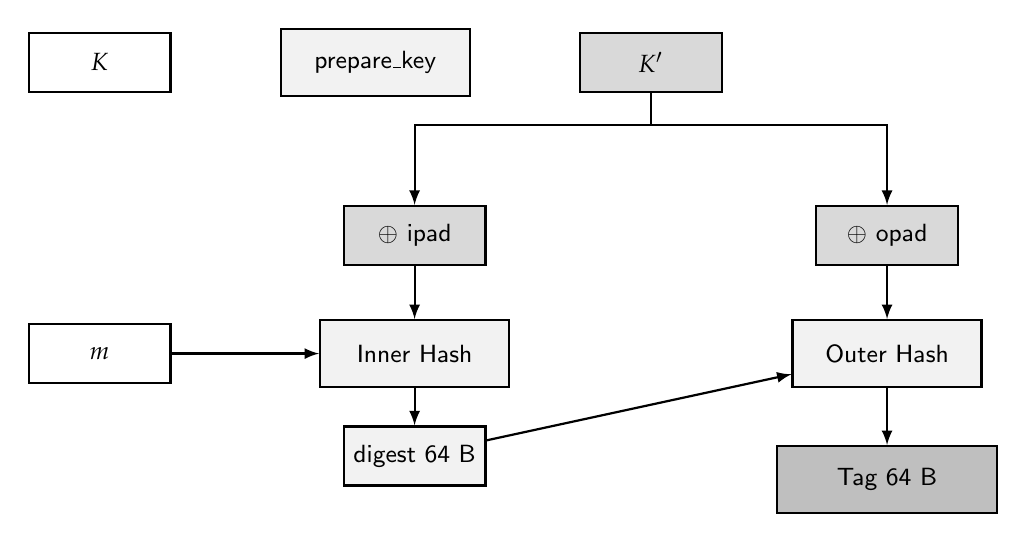
\begin{tikzpicture}[
			node distance=0.7cm and 1cm,
			box/.style={rectangle, draw=black, thick, fill=black!5, minimum width=2.4cm, minimum height=0.85cm, align=center, font=\sffamily\small},
			op/.style={rectangle, draw=black, thick, fill=black!15, minimum width=1.8cm, minimum height=0.75cm, align=center, font=\sffamily\small},
			input/.style={rectangle, draw=black, thick, fill=white, minimum width=1.8cm, minimum height=0.75cm, align=center, font=\sffamily\small},
			tagbox/.style={rectangle, draw=black, thick, fill=black!25, minimum width=2.8cm, minimum height=0.85cm, align=center, font=\sffamily\small},
			line/.style={draw, thick, -latex}
		]
		% Baris 1: input kunci dan persiapan
		\node[input] (k) at (0, 5) {$K$};
		\node[box] (prep) at (3.5, 5) {prepare\_key};
		\node[op] (kp) at (7, 5) {$K'$};

		% Titik percabangan dari K' ke dua XOR
		\coordinate (split) at (7, 4.2);
		\draw[thick] (kp.south) -- (split);

		% Baris 2: dua cabang XOR sejajar
		\node[op] (ipad) at (4, 2.8) {$\oplus$ ipad};
		\node[op] (opad) at (10, 2.8) {$\oplus$ opad};
		\draw[line] (split) -| (ipad.north);
		\draw[line] (split) -| (opad.north);

		% Baris 3: input pesan dan inner hash
		\node[input] (m) at (0, 1.3) {$m$};
		\node[box] (inner) at (4, 1.3) {Inner Hash};
		\draw[line] (ipad) -- (inner);
		\draw[line] (m) -- (inner);

		% Baris 4: digest
		\node[op, fill=black!5] (digest) at (4, 0) {digest 64 B};
		\draw[line] (inner) -- (digest);

		% Baris 4 paralel: outer hash
		\node[box] (outer) at (10, 1.3) {Outer Hash};
		\draw[line] (opad) -- (outer);
		\draw[line] (digest) -- (outer);

		% Tag
		\node[tagbox] (tag) at (10, -0.3) {Tag 64 B};
		\draw[line] (outer) -- (tag);
	\end{tikzpicture}
	\caption{Alur HMAC-SHA512 dalam tata letak grid: jalur kunci di atas, jalur pesan di bawah, konvergensi di outer hash.}
	\label{fig:hmac-overview}
\end{figure}

Cara membaca Gambar~\ref{fig:hmac-overview}: gambar ini tersusun dalam lima baris horizontal yang disusun vertikal. Baris teratas berisi tiga kotak: kunci $K$, kotak prepare\_key, dan $K'$. Dari $K'$ ada titik percabangan yang menurun ke baris kedua. Baris kedua berisi dua kotak sejajar: $\oplus$ ipad di posisi kiri dan $\oplus$ opad di posisi kanan. Baris ketiga berisi pesan $m$ di posisi paling kiri, inner hash di posisi tengah kiri sejajar dengan $\oplus$ ipad, dan outer hash di posisi tengah kanan sejajar dengan $\oplus$ opad. Baris keempat berisi digest 64 byte di bawah inner hash, dan tag 64 byte di bawah outer hash. Setiap panah mengalir ke bawah atau ke kanan tanpa silang. Inti pesan gambar ini adalah dua jalur paralel yang bertemu di outer hash: jalur kiri membawa kunci melalui prepare\_key dan ipad; jalur kanan membawa digest inner melalui opad; keduanya menghasilkan tag.

\subsection{Mengapa Tidak Cukup $H(K \parallel m)$}

Pendekatan naif untuk autentikasi pesan adalah $H(K \parallel m)$, yaitu mendahulukan kunci sebelum pesan. Ini terlihat aman karena kunci rahasia menjadi bagian dari input. Tetapi pendekatan ini rentan terhadap serangan length extension.

Serangan length extension adalah teknik di mana penyerang yang sudah memiliki $H(K \parallel m)$ dapat menghitung $H(K \parallel m \parallel \text{pad} \parallel m')$ tanpa perlu mengetahui $K$. Teknik ini bekerja karena SHA-512 (dan semua fungsi hash Merkle-Damgård) memproses input dalam blok, dan state internal setelah blok terakhir bisa dilanjutkan seolah-olah kita tahu apa yang diproses sebelumnya. Penyerang hanya perlu mengetahui hash dari pesan lama dan panjang pesan lama.

\subsection{Mengapa Tidak Cukup $H(m \parallel K)$}

Pendekatan kedua adalah $H(m \parallel K)$, yaitu menaruh kunci setelah pesan. Ini lebih kuat daripada $H(K \parallel m)$ karena penyerang tidak bisa menambahkan ekstensi di akhir. Tetapi pendekatan ini tetap bermasalah untuk alasan yang berbeda.

Fungsi hash Merkle-Damgård punya cacat teoretis ketika state internal bisa dikendalikan. Jika seorang penyerang bisa menemukan dua pesan $m_1$ dan $m_2$ sedemikian rupa sehingga setelah pemrosesan kedua pesan itu state internal hash-nya sama, maka $H(m_1 \parallel K) = H(m_2 \parallel K)$ untuk kunci apa pun. Ini disebut collision pada prefix.

\subsection{Mengapa HMAC Kuat}

HMAC mengatasi kedua masalah di atas dengan membungkus pesan dalam dua lapis hash yang berbeda. Lapisan dalam menghitung $H((K' \oplus \text{ipad}) \parallel m)$. Lapisan luar menghitung $H((K' \oplus \text{opad}) \parallel H_{\text{inner}})$. Serangan length extension pada lapisan dalam tidak membantu penyerang karena lapisan luar tetap harus dihitung, dan lapisan luar membutuhkan kunci yang sudah di-XOR dengan \texttt{opad} yang berbeda.

Tabel~\ref{tab:naive-vs-hmac} merangkum perbandingan keempat pendekatan.

\begin{table}[H]
	\centering
	\caption{Perbandingan pendekatan autentikasi pesan.}
	\label{tab:naive-vs-hmac}
	\footnotesize
	\begin{tabularx}{\textwidth}{l X X}
		\toprule
		Pendekatan                     & Kekuatan                                  & Kelemahan                                     \\
		\midrule
		$H(K \parallel m)$             & sederhana                                 & rentan length extension                       \\
		$H(m \parallel K)$             & kebal length extension                    & collision pada prefix melanggar jaminan       \\
		$H(K \parallel m \parallel K)$ & lebih kuat dari dua di atas               & pembuktian formal lemah, dua kali hash kunci  \\
		HMAC                           & pembuktian formal, praktis tahan serangan & dua kali hash, lebih lambat dari hash tunggal \\
		\bottomrule
	\end{tabularx}
\end{table}

Baris terakhir menjadi pilihan standar industri sejak RFC 2104 dipublikasikan pada 1997. HMAC sekarang menjadi wajib pada TLS 1.3, IPsec, dan SSH.

\section{Normalisasi Kunci}

\subsection{Tiga Jalur Eksekusi}

Fungsi \texttt{prepare\_key} menerima kunci dengan panjang berapa pun dan menghasilkan array 128 byte yang sudah dinormalisasi. Normalisasi berbeda berdasarkan panjang input.

Kunci yang lebih panjang dari 128 byte di-hash terlebih dahulu dengan SHA-512, menghasilkan 64 byte, lalu di-pad dengan nol hingga 128 byte. Kunci yang sama dengan 128 byte dipakai apa adanya. Kunci yang lebih pendek dari 128 byte di-pad dengan nol hingga 128 byte.

Gambar~\ref{fig:prepare-key} menampilkan **struktur pohon tiga cabang** dengan jalur konvergen di bagian bawah. Setiap cabang mengikuti panah vertikal lurus; jalur panjang memiliki satu langkah tambahan sebelum konvergen.

\begin{figure}[H]
	\centering
	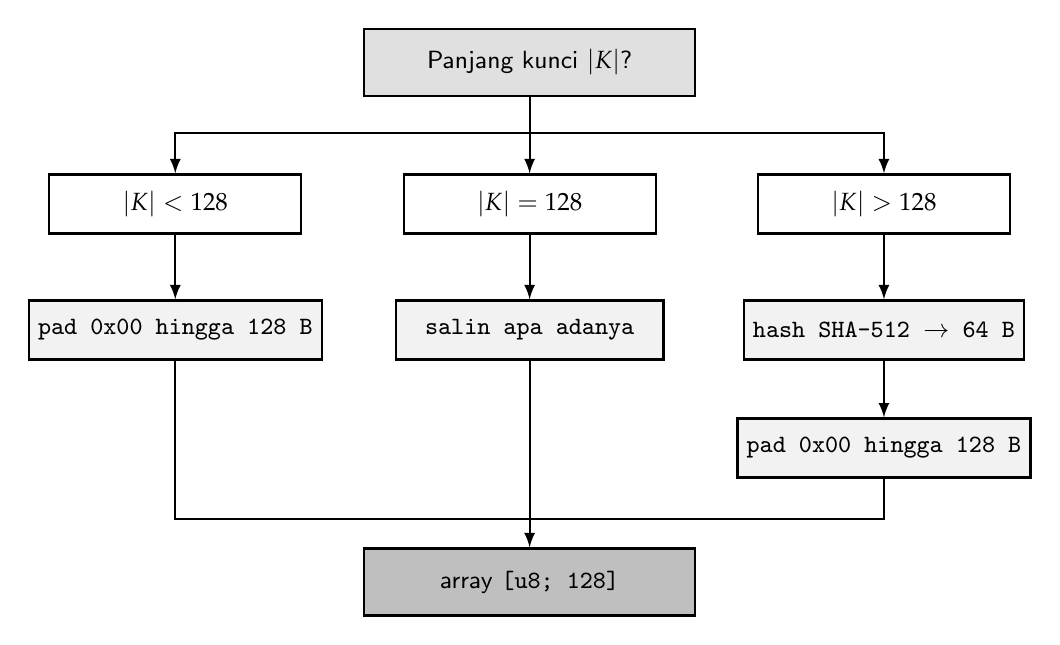
\begin{tikzpicture}[
			node distance=0.6cm and 1.2cm,
			qbox/.style={rectangle, draw=black, thick, fill=black!12, minimum width=4.2cm, minimum height=0.85cm, align=center, font=\sffamily\small},
			branch/.style={rectangle, draw=black, thick, fill=white, minimum width=3.2cm, minimum height=0.75cm, align=center, font=\sffamily\small},
			ans/.style={rectangle, draw=black, thick, fill=black!5, minimum width=3.4cm, minimum height=0.75cm, align=center, font=\ttfamily\small},
			result/.style={rectangle, draw=black, thick, fill=black!25, minimum width=4.2cm, minimum height=0.85cm, align=center, font=\sffamily\small},
			line/.style={draw, thick, -latex}
		]
		% Baris 0: pertanyaan
		\node[qbox] (q) at (0, 4) {Panjang kunci $|K|$?};

		% Baris 1: tiga cabang sejajar
		\node[branch] (lt) at (-4.5, 2.2) {$|K| < 128$};
		\node[branch] (eq) at (0, 2.2) {$|K| = 128$};
		\node[branch] (gt) at (4.5, 2.2) {$|K| > 128$};

		% Baris 2: jawaban
		\node[ans] (lt1) at (-4.5, 0.6) {pad \texttt{0x00} hingga 128 B};
		\node[ans] (eq1) at (0, 0.6) {salin apa adanya};
		\node[ans] (gt1) at (4.5, 0.6) {hash SHA-512 $\to$ 64 B};
		\node[ans] (gt2) at (4.5, -0.9) {pad \texttt{0x00} hingga 128 B};

		% Baris 3: konvergensi
		\node[result] (res) at (0, -2.6) {array \texttt{[u8; 128]}};

		% Panah pertanyaan ke cabang
		\coordinate (qbr) at (0, 3.1);
		\draw[thick] (q.south) -- (qbr);
		\draw[line] (qbr) -| (lt.north);
		\draw[line] (qbr) -- (eq.north);
		\draw[line] (qbr) -| (gt.north);

		% Panah cabang ke jawaban
		\draw[line] (lt.south) -- (lt1.north);
		\draw[line] (eq.south) -- (eq1.north);
		\draw[line] (gt.south) -- (gt1.north);
		\draw[line] (gt1.south) -- (gt2.north);

		% Konvergensi
		\coordinate (conv) at (0, -1.8);
		\draw[thick] (lt1.south) -- (lt1.south |- conv) -- (conv);
		\draw[thick] (eq1.south) -- (conv);
		\draw[thick] (gt2.south) -- (gt2.south |- conv) -- (conv);
		\draw[line] (conv) -- (res.north);
	\end{tikzpicture}
	\caption{Tiga jalur eksekusi \texttt{prepare\_key} berdasarkan panjang kunci. Semua jalur konvergen ke satu array 128 byte.}
	\label{fig:prepare-key}
\end{figure}

Cara membaca Gambar~\ref{fig:prepare-key}: gambar ini menampilkan struktur pohon simetris. Kotak paling atas berisi pertanyaan "Panjang kunci?". Kotak ini bercabang menjadi tiga cabang horizontal sejajar di baris kedua: $|K| < 128$ di kiri, $|K| = 128$ di tengah, dan $|K| > 128$ di kanan. Dari ketiga cabang, panah turun ke baris ketiga yang berisi jawaban masing-masing. Cabang kanan memiliki satu langkah tambahan (pad setelah hash) sehingga jawabannya dua tingkat. Ketiga jalur kemudian konvergen di titik tengah bawah (koordinat $(0, -1.8)$) sebelum masuk ke kotak hasil "array \texttt{[u8; 128]}". Tidak ada panah yang melintasi kotak lain. Inti pesan gambar ini adalah tiga jalur berbeda tetap bermuara pada satu hasil yang sama: array 128 byte.

\subsection{Jalur 1: Kunci Pendek}

Kunci yang lebih pendek dari 128 byte disalin ke awal array 128 byte yang sudah diinisialisasi dengan nol. Sisa array tetap nol.

\begin{lstlisting}[style=code]
fn prepare_key(key: &[u8]) -> [u8; 128] {
    let mut block_key = [0_u8; 128];
    if key.len() > 128 {
        let hash = zeroize::Zeroizing::new(Hash::hash(key));
        let hash_bytes = &*hash;
        block_key[..64].copy_from_slice(&hash_bytes[..64]);
    } else {
        block_key[..key.len()].copy_from_slice(key);
    }
    block_key
}
\end{lstlisting}

Contoh: kunci \texttt{b"secret"} sepanjang 6 byte menjadi array 128 byte dengan enam byte pertama berisi \texttt{73 65 63 72 65 74} dan 122 byte sisanya berisi nol.

\subsection{Jalur 2: Kunci Tepat 128 Byte}

Kunci yang panjangnya tepat 128 byte disalin apa adanya. Tidak ada padding, tidak ada hash.

\subsection{Jalur 3: Kunci Panjang}

Kunci yang lebih panjang dari 128 byte di-hash terlebih dahulu dengan SHA-512, menghasilkan digest 64 byte. Digest ini ditempatkan di awal array 128 byte, sisa 64 byte diisi nol. Proses ini membuang sebagian besar entropi kunci, tetapi memenuhi persyaratan RFC 2104 dan menjaga konsistensi ukuran kunci efektif.

Perhatikan bahwa hash hasil kunci panjang dibungkus dalam \texttt{Zeroizing}. Ini penting karena digest antara adalah turunan langsung dari kunci rahasia. Tanpa zeroization, digest bisa tertinggal di stack setelah fungsi selesai. \texttt{Zeroizing} memastikan memori dihapus dengan operasi write yang tidak dapat dioptimasi oleh compiler.

\subsection{Mengapa Tiga Jalur, Bukan Satu}

Satu-satunya jalur yang benar-benar diperlukan oleh RFC 2104 adalah jalur hash untuk kunci yang lebih panjang dari blok. Tetapi ada tiga alasan mengapa implementasi modern memilih tiga jalur.

Pertama, performa. Hash SHA-512 memakan waktu jauh lebih lama daripada padding nol. Untuk kunci yang sudah pendek, tidak ada alasan untuk menghitung hash.

Kedua, determinisme. RFC 2104 menentukan bahwa kunci pendek di-pad dengan nol, bukan di-hash. Implementasi yang selalu menghitung hash akan menghasilkan tag yang berbeda untuk kunci pendek yang sama, dan tidak kompatibel dengan implementasi lain.

Ketiga, keamanan. Kunci dengan panjang tepat 128 byte adalah kasus paling efisien, karena tidak ada padding dan tidak ada hash.

Tabel~\ref{tab:key-cases} merangkum tiga jalur.

\begin{table}[H]
	\centering
	\caption{Tiga jalur \texttt{prepare\_key} dan hasilnya.}
	\label{tab:key-cases}
	\small
	\begin{tabularx}{\textwidth}{l X l}
		\toprule
		Panjang kunci & Operasi                               & Ukuran setelah \\
		\midrule
		$< 128$ byte  & salin ke array nol, sisanya tetap nol & 128 byte       \\
		$= 128$ byte  & salin apa adanya                      & 128 byte       \\
		$> 128$ byte  & hash SHA-512 (64 byte), lalu pad nol  & 128 byte       \\
		\bottomrule
	\end{tabularx}
\end{table}

\subsection{Kesalahan yang Sering Terjadi}

Implementasi yang salah sering memakai jalur hash untuk semua kunci. Ini menghasilkan tag yang tidak kompatibel dengan implementasi standar. Pada test vector RFC 4231 dengan kunci \texttt{0x0b} yang diulang 20 kali (panjang 20 byte), implementasi yang salah akan menghitung hash dari 20 byte tersebut sebelum padding, menghasilkan tag yang berbeda.

Implementasi yang salah juga sering tidak membungkus hasil hash dalam \texttt{Zeroizing}. Ini meninggalkan jejak digest antara di stack, yang bisa dibaca oleh serangan memory disclosure seperti Heartbleed.

\section{Pembentukan ipad dan opad}

\subsection{Konstanta 0x36 dan 0x5c}

RFC 2104 memilih dua konstanta yang berbeda jauh secara bit: \texttt{ipad} = \texttt{0x36} (biner \texttt{00110110}) dan \texttt{opad} = \texttt{0x5c} (biner \texttt{01011100}). Pilihan ini bukan sembarang. Hamming distance antara kedua konstanta adalah 4 bit dari 8, yang berarti sekitar setengah bit berbeda.

Alasan pemilihan ini adalah untuk memastikan bahwa proses hash inner dan outer benar-benar berbeda. Jika \texttt{ipad} dan \texttt{opad} hanya berbeda satu atau dua bit, ada kemungkinan secara teoretis bahwa serangan tertentu bisa menemukan hubungan antar dua proses. Dengan perbedaan setengah bit, kedua proses menjadi fungsi hash yang tidak berkorelasi secara praktis.

Gambar~\ref{fig:ipad-opad-bits} menyajikan ketiga nilai dalam **tabel bit 8 kolom** dengan header posisi bit di bagian atas, label baris di bagian kiri, dan separator horizontal antar baris.

\begin{figure}[H]
	\centering
	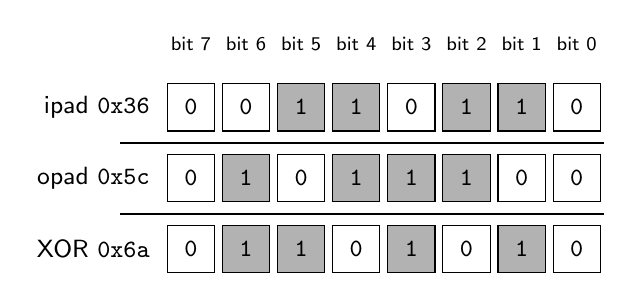
\begin{tikzpicture}[
			bit/.style={rectangle, draw=black, minimum width=0.6cm, minimum height=0.6cm, font=\ttfamily\small, align=center},
			bit1/.style={bit, fill=black!30},
			hdr/.style={font=\scriptsize\sffamily, anchor=south},
			lbl/.style={font=\sffamily\small, anchor=east}
		]
		% Header posisi bit
		\node[hdr] at (0, 1.5) {bit 7};
		\node[hdr] at (0.7, 1.5) {bit 6};
		\node[hdr] at (1.4, 1.5) {bit 5};
		\node[hdr] at (2.1, 1.5) {bit 4};
		\node[hdr] at (2.8, 1.5) {bit 3};
		\node[hdr] at (3.5, 1.5) {bit 2};
		\node[hdr] at (4.2, 1.5) {bit 1};
		\node[hdr] at (4.9, 1.5) {bit 0};

		% Baris 1: ipad 0x36 = 0011 0110
		\node[lbl] at (-0.4, 0.9) {ipad \texttt{0x36}};
		\node[bit]  at (0, 0.9) {0};
		\node[bit]  at (0.7, 0.9) {0};
		\node[bit1] at (1.4, 0.9) {1};
		\node[bit1] at (2.1, 0.9) {1};
		\node[bit]  at (2.8, 0.9) {0};
		\node[bit1] at (3.5, 0.9) {1};
		\node[bit1] at (4.2, 0.9) {1};
		\node[bit]  at (4.9, 0.9) {0};

		% Baris 2: opad 0x5c = 0101 1100
		\node[lbl] at (-0.4, 0) {opad \texttt{0x5c}};
		\node[bit]  at (0, 0) {0};
		\node[bit1] at (0.7, 0) {1};
		\node[bit]  at (1.4, 0) {0};
		\node[bit1] at (2.1, 0) {1};
		\node[bit1] at (2.8, 0) {1};
		\node[bit1] at (3.5, 0) {1};
		\node[bit]  at (4.2, 0) {0};
		\node[bit]  at (4.9, 0) {0};

		% Baris 3: XOR 0x6a = 0110 1010
		\node[lbl] at (-0.4, -0.9) {XOR \texttt{0x6a}};
		\node[bit]  at (0, -0.9) {0};
		\node[bit1] at (0.7, -0.9) {1};
		\node[bit1] at (1.4, -0.9) {1};
		\node[bit]  at (2.1, -0.9) {0};
		\node[bit1] at (2.8, -0.9) {1};
		\node[bit]  at (3.5, -0.9) {0};
		\node[bit1] at (4.2, -0.9) {1};
		\node[bit]  at (4.9, -0.9) {0};

		% Separator
		\draw[thick] (-0.9, 0.45) -- (5.25, 0.45);
		\draw[thick] (-0.9, -0.45) -- (5.25, -0.45);
	\end{tikzpicture}
	\caption{Representasi bit-level ipad, opad, dan XOR di antaranya. Baris 1 dan 2 berbeda di empat posisi bit; baris 3 adalah XOR bit-per-bit.}
	\label{fig:ipad-opad-bits}
\end{figure}

Cara membaca Gambar~\ref{fig:ipad-opad-bits}: gambar ini tersusun sebagai tabel bit 3 baris dan 8 kolom. Delapan kolom diberi header dari "bit 7" di kiri sampai "bit 0" di kanan, dengan posisi bit 7 sebagai most significant bit dan bit 0 sebagai least significant bit. Baris pertama berlabel "ipad 0x36" berisi pola 0-0-1-1-0-1-1-0. Baris kedua berlabel "opad 0x5c" berisi pola 0-1-0-1-1-1-0-0. Baris ketiga berlabel "XOR 0x6a" berisi pola 0-1-1-0-1-0-1-0. Sel yang bernilai 1 diberi latar abu-abu gelap, sedangkan sel yang bernilai 0 berlatar putih. Garis horizontal tipis memisahkan setiap baris. Inti pesan gambar ini adalah ipad dan opad berbeda secara substansial pada empat posisi bit, dan XOR di antara keduanya menghasilkan konstanta 0x6a.

\subsection{Konstruksi HMAC::new}

Fungsi \texttt{HMAC::new} menerima kunci, memanggil \texttt{prepare\_key}, membentuk \texttt{ipad} yang sudah di-XOR dengan kunci, memulai inner hash, lalu menyimpan state.

\begin{lstlisting}[style=code]
pub fn new(key: impl AsRef<[u8]>) -> Self {
    let key = key.as_ref();
    let mut block_key = Self::prepare_key(key);
    let mut padded = [0x36_u8; 128];
    for (padded_byte, block_byte)
        in padded.iter_mut().zip(block_key.iter())
    {
        *padded_byte ^= *block_byte;
    }
    let mut ih = Hash::new();
    ih.update(&padded);
    zeroize::Zeroize::zeroize(&mut block_key);
    HMAC {
        ih: Some(ih),
        padded,
    }
}
\end{lstlisting}

Poin-poin penting. Array \texttt{padded} diinisialisasi dengan \texttt{0x36} di setiap byte. Setiap byte di-XOR dengan byte yang sesuai dari \texttt{block\_key}. Hasilnya adalah \texttt{0x36 XOR K'} untuk setiap byte, yang sesuai dengan rumus RFC 2104. Hasher \texttt{ih} (inner hasher) dimulai dengan state SHA-512 yang sudah memproses 128 byte padding. Setelah \texttt{ih} disiapkan, \texttt{block\_key} di-zeroize karena sudah tidak diperlukan. Struct \texttt{HMAC} menyimpan dua hal: hasher inner yang sudah setengah jalan, dan array \texttt{padded} yang berisi \texttt{0x36 XOR K'}.

\subsection{State yang Disimpan}

Setelah \texttt{new}, struct \texttt{HMAC} berisi dua field. Field \texttt{ih} adalah \texttt{Option<Hash>} yang menyimpan hasher inner yang sudah memproses \texttt{ipad}. Field \texttt{padded} adalah \texttt{[u8; 128]} yang berisi \texttt{0x36 XOR K'}.

Gambar~\ref{fig:hmac-struct} menampilkan layout memori struct dalam **kotak berbingkai** dengan dua field yang disejajarkan secara horizontal. Setiap field diberi label di dalam kotak dan keterangan tambahan di bawahnya.

\begin{figure}[H]
	\centering
	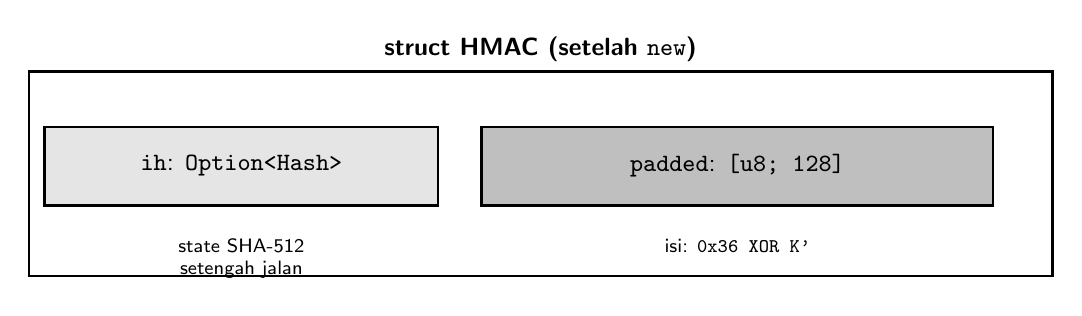
\begin{tikzpicture}[
			frame/.style={rectangle, draw=black, thick},
			field/.style={rectangle, draw=black, thick, minimum height=1.0cm, align=center, font=\sffamily\small},
			note/.style={font=\scriptsize\sffamily, anchor=north, align=center}
		]
		% Bingkai luar
		\draw[thick] (-5.5, 1.3) rectangle (7.5, -1.3);

		% Judul
		\node[font=\sffamily\small\bfseries, anchor=south] at (1, 1.3) {struct HMAC (setelah \texttt{new})};

		% Field 1: ih
		\node[field, fill=black!10, minimum width=5cm] (ih) at (-2.8, 0.1) {\texttt{ih}: \texttt{Option<Hash>}};
		\node[note] at (-2.8, -0.7) {state SHA-512\\setengah jalan};

		% Field 2: padded
		\node[field, fill=black!25, minimum width=6.5cm] (pad) at (3.5, 0.1) {\texttt{padded}: \texttt{[u8; 128]}};
		\node[note] at (3.5, -0.7) {isi: \texttt{0x36 XOR K'}};
	\end{tikzpicture}
	\caption{Layout memori struct \texttt{HMAC} setelah \texttt{new}: dua field berdampingan di dalam bingkai.}
	\label{fig:hmac-struct}
\end{figure}

Cara membaca Gambar~\ref{fig:hmac-struct}: gambar ini menampilkan satu kotak persegi panjang besar sebagai bingkai luar, dengan judul "struct HMAC (setelah new)" di atasnya. Di dalam bingkai ada dua kotak kecil berdampingan secara horizontal. Kotak kiri lebih sempit, berlabel "ih: Option<Hash>" dengan latar abu-abu muda, dan di bawahnya ada keterangan "state SHA-512 setengah jalan". Kotak kanan lebih lebar, berlabel "padded: [u8; 128]" dengan latar abu-abu lebih gelap, dan di bawahnya ada keterangan "isi: 0x36 XOR K'". Kedua kotak sejajar di tengah bingkai. Inti pesan gambar ini adalah struct HMAC menyimpan dua field dengan peran berbeda: state hash setengah jalan untuk inner, dan array padding yang akan ditransformasi di finalize.

\subsection{Ringkasan}

\begin{table}[H]
	\centering
	\caption{Perbandingan ipad dan opad.}
	\label{tab:ipad-opad}
	\small
	\begin{tabularx}{\textwidth}{l l X}
		\toprule
		Aspek               & ipad                            & opad                                 \\
		\midrule
		Nilai byte          & \texttt{0x36}                   & \texttt{0x5c}                        \\
		Biner               & \texttt{00110110}               & \texttt{01011100}                    \\
		Panjang             & 128 byte (block size SHA-512)   & 128 byte                             \\
		Kapan dipakai       & awal inner hash di \texttt{new} & awal outer hash di \texttt{finalize} \\
		Panjang setelah XOR & 128 byte                        & 128 byte                             \\
		\bottomrule
	\end{tabularx}
\end{table}

\section{Transformasi 0x6a: Trik Kunci}

\subsection{Masalah yang Harus Dipecahkan}

Saat \texttt{finalize} dipanggil, kita perlu menghitung outer hash yang membutuhkan \texttt{opad XOR K'}. Tetapi struct hanya menyimpan \texttt{ipad XOR K'}, bukan \texttt{K'} secara terpisah. Ada dua pendekatan naif untuk mendapatkan \texttt{opad XOR K'}.

Pendekatan pertama adalah menyimpan \texttt{K'} di struct. Ini menambah 128 byte per konteks HMAC. Pendekatan kedua adalah menyimpan dua array: \texttt{ipad XOR K'} dan \texttt{opad XOR K'}. Ini menambah 128 byte lagi.

libvctrl memilih pendekatan ketiga: mengubah \texttt{ipad XOR K'} menjadi \texttt{opad XOR K'} secara in-place dengan satu operasi XOR.

\subsection{Aljabar XOR}

Aljabar yang membuat ini bekerja sangat sederhana. Misalkan $p$ adalah array yang berisi $\text{ipad} \oplus K'$. Kita ingin mengubahnya menjadi array yang berisi $\text{opad} \oplus K'$. Yang perlu dilakukan adalah meng-XOR setiap byte dengan suatu konstanta $c$:

\[
	p \oplus c = (\text{ipad} \oplus K') \oplus c
\]

Kita ingin hasilnya sama dengan $\text{opad} \oplus K'$:

\[
	(\text{ipad} \oplus K') \oplus c = \text{opad} \oplus K'
\]

Kedua sisi di-XOR dengan $K'$:

\[
	\text{ipad} \oplus c = \text{opad}
\]

Kedua sisi di-XOR dengan $\text{ipad}$:

\[
	c = \text{ipad} \oplus \text{opad} = \texttt{0x36} \oplus \texttt{0x5c} = \texttt{0x6a}
\]

Gambar~\ref{fig:0x6a-derivation} menyajikan derivasi ini sebagai **lima langkah vertikal** dari atas ke bawah, dengan setiap langkah menempati satu kotak dan panah konstan mengalir dari satu langkah ke langkah berikutnya.

\begin{figure}[H]
	\centering
	\begin{tikzpicture}[
			step/.style={rectangle, draw=black, thick, fill=black!5, minimum width=10cm, minimum height=0.85cm, align=center, font=\ttfamily\small},
			steplbl/.style={font=\sffamily\small, anchor=east, align=right},
			line/.style={draw, thick, -latex}
		]
		\node[step, fill=black!10] (s1) at (0, 3.5) {Langkah 1: ipad $=$ \texttt{0x36} (diulang 128$\times$), opad $=$ \texttt{0x5c}};
		\node[step] (s2) at (0, 2) {Langkah 2: $c = \text{ipad} \oplus \text{opad} = \texttt{0x36} \oplus \texttt{0x5c} = \texttt{0x6a}$};
		\node[step] (s3) at (0, 0.5) {Langkah 3: $(\text{ipad} \oplus K') \oplus c = (\texttt{0x36} \oplus K') \oplus \texttt{0x6a}$};
		\node[step] (s4) at (0, -1) {Langkah 4: $= \texttt{0x36} \oplus K' \oplus \texttt{0x36} \oplus \texttt{0x5c} = K' \oplus \texttt{0x5c}$};
		\node[step, fill=black!20] (s5) at (0, -2.5) {Hasil: $= \text{opad} \oplus K'$ \quad (padding outer siap)} ;

		\draw[line] (s1) -- (s2);
		\draw[line] (s2) -- (s3);
		\draw[line] (s3) -- (s4);
		\draw[line] (s4) -- (s5);
	\end{tikzpicture}
	\caption{Derivasi konstanta transformasi \texttt{0x6a} dalam lima langkah aljabar vertikal.}
	\label{fig:0x6a-derivation}
\end{figure}

Cara membaca Gambar~\ref{fig:0x6a-derivation}: gambar ini menampilkan lima kotak persegi panjang yang tersusun vertikal dari atas ke bawah. Kotak pertama berisi definisi awal ipad dan opad. Kotak kedua berisi perhitungan konstanta $c$ sebagai XOR dari kedua padding. Kotak ketiga menerapkan $c$ ke array yang sudah mengandung $K'$. Kotak keempat menyederhanakan aljabar dengan mengelompokkan dua suku ipad yang saling meniadakan (XOR dengan dirinya sendiri menghasilkan nol). Kotak kelima berisi hasil akhir: padding outer siap dipakai. Panah pendek menghubungkan setiap kotak ke kotak berikutnya dari atas ke bawah. Kotak terakhir diberi latar abu-abu lebih gelap untuk menandai hasil akhir. Inti pesan gambar ini adalah transformasi 0x6a adalah konsekuensi langsung dari sifat asosiatif dan identitas XOR, bukan trik ad-hoc.

\subsection{Implementasi di finalize}

Kode pada \texttt{finalize} sangat ringkas.

\begin{lstlisting}[style=code]
pub fn finalize(mut self) -> [u8; 64] {
    for padded_byte in self.padded.iter_mut() {
        *padded_byte ^= 0x6a;
    }
    let mut oh = Hash::new();
    oh.update(&self.padded);
    let inner = zeroize::Zeroizing::new(
        self.ih
            .take()
            .unwrap_or_else(|| Hash::new())
            .finalize(),
    );
    oh.update(&*inner);
    oh.finalize()
}
\end{lstlisting}

Langkah pertama mengubah \texttt{padded} dari \texttt{0x36 XOR K'} menjadi \texttt{0x5c XOR K'} lewat satu loop yang meng-XOR setiap byte dengan \texttt{0x6a}. Setelah loop ini selesai, \texttt{padded} sudah berisi padding outer yang siap dipakai.

Langkah kedua memulai hasher outer \texttt{oh} dan memproses \texttt{padded} yang sudah ditransformasi. Ini setara dengan menjalankan outer hash dengan prefix \texttt{opad XOR K'}.

Langkah ketiga mengambil hasher inner dari \texttt{self.ih} (lewat \texttt{take} yang memindahkan isi Option), menyelesaikannya, dan membungkus digest yang dihasilkan dalam \texttt{Zeroizing} agar nanti dihapus dari memori.

Langkah keempat memproses digest inner ke dalam hasher outer. Langkah kelima menyelesaikan hasher outer dan mengembalikan tag 64 byte.

\subsection{Penghematan Memori}

Perbedaan antara menyimpan \texttt{K'} secara terpisah versus mentransformasi \texttt{padded} secara in-place cukup signifikan pada skala besar. Tabel~\ref{tab:memory-savings} menunjukkan perbandingannya.

\begin{table}[H]
	\centering
	\caption{Perbandingan memori dua pendekatan finalize.}
	\label{tab:memory-savings}
	\small
	\begin{tabularx}{\textwidth}{l r r r}
		\toprule
		Pendekatan                  & Per konteks & 100 konteks & 1000 konteks \\
		\midrule
		Simpan \texttt{K'} terpisah & 256 byte    & 25,6 KB     & 256 KB       \\
		Transformasi \texttt{0x6a}  & 128 byte    & 12,8 KB     & 128 KB       \\
		\bottomrule
	\end{tabularx}
\end{table}

Selisih 128 byte per konteks mungkin tidak signifikan pada aplikasi yang menjalankan satu HMAC pada satu waktu. Tetapi pada server yang memproses ribuan koneksi TLS secara paralel, di mana setiap koneksi memiliki setidaknya satu konteks HMAC aktif, selisih ini bisa mencapai ratusan kilobyte. Pada sistem embedded dengan memori terbatas, selisih ini bisa menjadi faktor penentu.

\subsection{Mengapa 0x6a, Bukan 0x5c XOR 0x36 Sendiri}

Beberapa pembaca mungkin bertanya mengapa kodenya tidak menulis ekspresi \texttt{0x5c \^ 0x36} secara langsung. Ada dua alasan.

Pertama, konstanta yang sudah dihitung \texttt{0x6a} lebih cepat dieksekusi. Meskipun \texttt{0x5c \^ 0x36} adalah operasi XOR dua konstanta yang akan dioptimasi oleh compiler menjadi satu konstanta, ada risiko compiler tidak melakukannya pada semua target. Menulis \texttt{0x6a} langsung menghilangkan risiko itu.

Kedua, \texttt{0x6a} lebih mudah dibaca dalam konteks. Pembaca yang mengenal trik ini akan langsung tahu bahwa loop tersebut mengubah \texttt{ipad} menjadi \texttt{opad}.

\subsection{Kompatibilitas dengan SHA-384}

Trik \texttt{0x6a} berlaku universal, bukan spesifik untuk SHA-512. Konstanta \texttt{ipad} dan \texttt{opad} yang ditentukan oleh RFC 2104 adalah \texttt{0x36} dan \texttt{0x5c} untuk semua fungsi hash, terlepas dari ukuran blok. Yang berbeda adalah panjang block size: 128 byte untuk SHA-512 dan SHA-384, 64 byte untuk SHA-256 dan SHA-224, 64 byte untuk SHA-1 dan MD5.

Implementasi SHA-384 di libvctrl memakai trik yang sama.

\begin{lstlisting}[style=code]
impl_hmac!(Hash, 48, 128);
\end{lstlisting}

Baris ini menginstansiasi \texttt{HMAC} dengan output 48 byte dan block size 128 byte. Konstanta \texttt{0x6a} tetap sama karena \texttt{ipad} dan \texttt{opad} tidak berubah.

\section{Finalize dan Pembentukan Tag}

\subsection{Alur Lengkap}

Fungsi \texttt{finalize} mengubah struct \texttt{HMAC} yang menyimpan state setengah jalan menjadi tag 64 byte. Gambar~\ref{fig:finalize-flow} menampilkan alur finalize dalam **dua baris paralel** yang bertemu di outer hash, tanpa panah diagonal.

\begin{figure}[H]
	\centering
	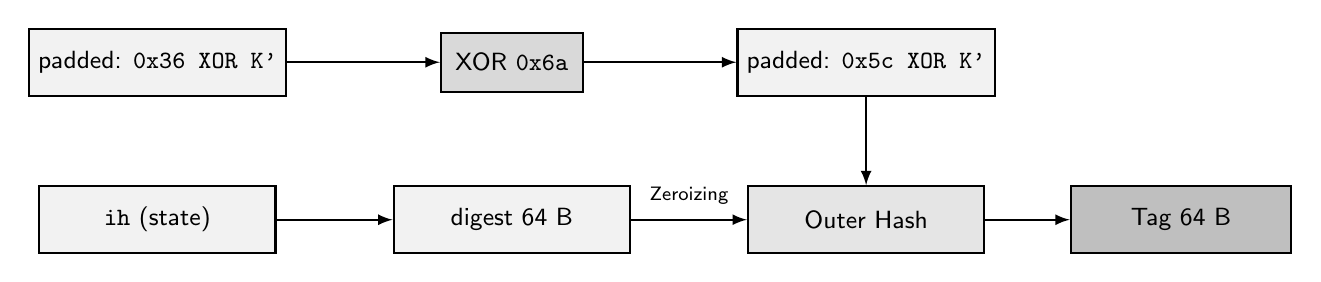
\begin{tikzpicture}[
			node distance=0.6cm and 1cm,
			box/.style={rectangle, draw=black, thick, fill=black!5, minimum width=3cm, minimum height=0.85cm, align=center, font=\sffamily\small},
			op/.style={rectangle, draw=black, thick, fill=black!15, minimum width=1.8cm, minimum height=0.75cm, align=center, font=\sffamily\small},
			outerbox/.style={rectangle, draw=black, thick, fill=black!10, minimum width=3cm, minimum height=0.85cm, align=center, font=\sffamily\small},
			tagbox/.style={rectangle, draw=black, thick, fill=black!25, minimum width=2.8cm, minimum height=0.85cm, align=center, font=\sffamily\small},
			line/.style={draw, thick, -latex}
		]
		% Baris atas: transformasi padding
		\node[box] (p1) at (0, 3) {padded: \texttt{0x36 XOR K'}};
		\node[op] (xor) at (4.5, 3) {XOR \texttt{0x6a}};
		\node[box] (p2) at (9, 3) {padded: \texttt{0x5c XOR K'}};

		% Baris bawah: state ih dan outer merge
		\node[box] (ih) at (0, 1) {\texttt{ih} (state)};
		\node[box] (dig) at (4.5, 1) {digest 64 B};
		\node[outerbox] (o) at (9, 1) {Outer Hash};
		\node[tagbox] (tag) at (13, 1) {Tag 64 B};

		% Panah baris atas
		\draw[line] (p1) -- (xor);
		\draw[line] (xor) -- (p2);

		% Panah baris bawah
		\draw[line] (ih) -- (dig);
		\draw[line] (dig) -- node[above=2pt, font=\scriptsize\sffamily] {Zeroizing} (o);
		\draw[line] (o) -- (tag);

		% Panah p2 ke o (vertikal)
		\draw[line] (p2.south) -- (o.north);
	\end{tikzpicture}
	\caption{Alur finalize: baris atas mentransformasi padding, baris bawah memproses digest, konvergensi di outer hash.}
	\label{fig:finalize-flow}
\end{figure}

Cara membaca Gambar~\ref{fig:finalize-flow}: gambar ini menampilkan dua baris horizontal yang sejajar. Baris atas berisi tiga kotak: padding dengan isi awal, operasi XOR 0x6a, dan padding dengan isi ter-transformasi. Baris bawah berisi empat kotak: state ih, digest 64 byte, outer hash, dan tag. Setiap kotak dihubungkan oleh panah horizontal ke kanan, dan panah dari kotak padding ter-transformasi (baris atas) turun vertikal ke outer hash (baris bawah). Panah dari digest ke outer hash diberi label "Zeroizing" di atasnya. Inti pesan gambar ini adalah outer hash menerima dua masukan: padding ter-transformasi dari baris atas, dan digest inner dari baris bawah; hasilnya adalah tag 64 byte.

\subsection{Pembentukan Inner Digest}

Inner hash sudah menyimpan state setengah jalan sejak \texttt{new}. Ketika \texttt{update} dipanggil satu atau beberapa kali, pesan ditambahkan ke state itu.

\begin{lstlisting}[style=code]
pub fn update(&mut self, input: impl AsRef<[u8]>) {
    if let Some(ref mut ih) = self.ih {
        ih.update(input);
    }
}
\end{lstlisting}

Panggilan \texttt{finalize} pada hasher inner menghasilkan digest 64 byte. Digest ini adalah $H(\text{ipad} \oplus K' \parallel m)$.

Karena digest ini adalah nilai antara yang sensitif, ia dibungkus dalam \texttt{Zeroizing}. \texttt{Zeroizing} adalah wrapper yang secara otomatis memanggil \texttt{zeroize} pada \texttt{Drop}. Ini memastikan memori yang menyimpan digest dihapus dengan operasi write yang tidak bisa dioptimasi oleh compiler.

\subsection{Pembentukan Outer Digest}

Setelah digest inner siap, fungsi \texttt{finalize} memanggil outer hash.

\begin{lstlisting}[style=code]
let mut oh = Hash::new();
oh.update(&self.padded);
oh.update(&*inner);
oh.finalize()
\end{lstlisting}

Tiga baris ini menghitung $H(\text{opad} \oplus K' \parallel \text{digest})$. Hasilnya adalah tag final 64 byte.

\subsection{Mengapa Dua Lapis Hash}

Konstruksi dua lapis hash bukan sekadar komplikasi. Ia adalah inti dari keamanan HMAC. Lapisan dalam menghitung hash pesan dengan padding ipad yang menempel pada kunci. Lapisan luar menghitung hash dari hasil lapisan dalam, dengan padding opad yang juga menempel pada kunci.

Jika serangan length extension berhasil pada lapisan dalam, penyerang masih harus menghitung lapisan luar dari awal. Lapisan luar tidak mengenal state internal lapisan dalam, karena lapisan luar dimulai dari state baru yang segar.

\section{Keamanan: Constant-Time dan Zeroization}

\subsection{Verifikasi Tag}

Setelah tag dihitung, langkah berikutnya adalah memverifikasi tag yang diterima dengan tag yang dihitung. Implementasi naif memakai perbandingan \texttt{==} biasa. Ini bermasalah karena perbandingan \texttt{==} pada slice byte biasanya berhenti di byte pertama yang berbeda. Pola waktu ini membocorkan informasi tentang berapa banyak byte prefix yang benar.

Serangan timing yang memanfaatkan kebocoran ini disebut timing attack. Untuk tag 64 byte, penyerang perlu mencoba rata-rata 32 kali per byte, total sekitar 2048 percobaan untuk memulihkan tag yang benar.

Solusinya adalah perbandingan constant-time. Perbandingan ini selalu memeriksa seluruh byte, terlepas dari apakah sudah ada perbedaan atau belum.

\begin{lstlisting}[style=code]
pub fn verify(x: &[u8], y: &[u8]) -> bool {
    let mut diff: u32 = 0;
    for (byte_x, byte_y) in x.iter().zip(y.iter()) {
        diff |= u32::from(byte_x ^ byte_y);
    }
    if x.len() != y.len() {
        diff |= 0xffff_ffff;
    }
    let diff = core::hint::black_box(diff);
    diff == 0
}
\end{lstlisting}

Tiga hal yang membuat fungsi ini constant-time. Pertama, perulangan tidak pernah berhenti lebih awal. Ia selalu memeriksa seluruh byte yang ada. Kedua, akumulasi memakai OR bit-wise, yang tidak mempersingkat perulangan pada perbedaan pertama. Ketiga, pengecekan panjang setelah perulangan memastikan bahwa perbedaan panjang juga terdeteksi, dan \texttt{black\_box} mencegah compiler mengoptimasi diff menjadi shortcut.

\subsection{Mask WASM}

Pada target WebAssembly, timing attack konvensional kurang relevan karena WebAssembly dijalankan dalam sandbox yang tidak membocorkan waktu eksekusi per instruksi ke JavaScript. Namun, ada serangan yang lebih halus yang memanfaatkan waktu wall-clock. Untuk mengatasinya, libvctrl menambahkan lapisan tambahan pada WASM.

\begin{lstlisting}[style=code]
#[cfg(any(target_arch = "wasm32", target_arch = "wasm64"))]
{
    let (mut hash_x, mut hash_y) = (0_u32, 0_u32);
    for (byte_x, byte_y) in x.iter().zip(y.iter()) {
        hash_x ^= (hash_x << 5)
            .wrapping_add((hash_x >> 2) ^ u32::from(*byte_x));
        hash_y ^= (hash_y << 5)
            .wrapping_add((hash_y >> 2) ^ u32::from(*byte_y));
    }
    diff |= hash_x ^ hash_y;
}
\end{lstlisting}

Kode ini menghitung hash dari setiap slice secara paralel dan menambahkan perbedaan hash ke akumulator. Tujuannya bukan untuk mencegah timing attack konvensional, tetapi untuk memperumit analisis waktu wall-clock di tingkat JavaScript. Teknik ini disebut hash-based blinding.

\subsection{Zeroization Lifecycle}

Data sensitif dalam HMAC ada di beberapa titik. Gambar~\ref{fig:zeroization} menampilkan lifecycle ini sebagai **timeline horizontal** dengan tiga batang "alive" yang berakhir di titik zeroization.

\begin{figure}[H]
	\centering
	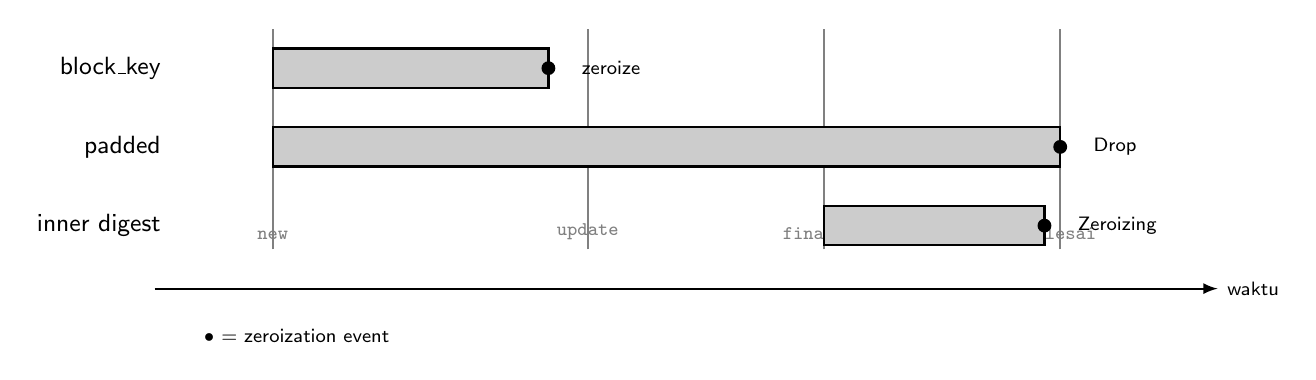
\begin{tikzpicture}[
			lbl/.style={font=\sffamily\small, anchor=east},
			phase/.style={font=\scriptsize\sffamily, anchor=south, gray}
		]
		% Garis waktu
		\draw[thick, -latex] (-0.5, -0.8) -- (13, -0.8);
		\node[font=\scriptsize\sffamily, anchor=west] at (13, -0.8) {waktu};

		% Penanda fase
		\foreach \x/\name in {1/{\texttt{new}}, 5/{\texttt{update}}, 8/{\texttt{finalize}}, 11/{\texttt{selesai}}} {
				\draw[thick, gray] (\x, -0.3) -- (\x, 2.5);
				\node[phase] at (\x, -0.3) {\name};
			}

		% Baris 1: block_key
		\node[lbl] at (-0.3, 2) {block\_key};
		\fill[black!20] (1, 1.75) rectangle (4.5, 2.25);
		\draw[thick] (1, 1.75) rectangle (4.5, 2.25);
		\fill[black] (4.5, 2) circle (2.5pt);
		\node[font=\scriptsize\sffamily, anchor=west] at (4.8, 2) {zeroize};

		% Baris 2: padded
		\node[lbl] at (-0.3, 1) {padded};
		\fill[black!20] (1, 0.75) rectangle (11, 1.25);
		\draw[thick] (1, 0.75) rectangle (11, 1.25);
		\fill[black] (11, 1) circle (2.5pt);
		\node[font=\scriptsize\sffamily, anchor=west] at (11.3, 1) {Drop};

		% Baris 3: inner digest
		\node[lbl] at (-0.3, 0) {inner digest};
		\fill[black!20] (8, -0.25) rectangle (10.8, 0.25);
		\draw[thick] (8, -0.25) rectangle (10.8, 0.25);
		\fill[black] (10.8, 0) circle (2.5pt);
		\node[font=\scriptsize\sffamily, anchor=west] at (11.1, 0) {Zeroizing};

		% Legenda
		\node[font=\scriptsize\sffamily, anchor=west] at (0, -1.4) {$\bullet$ = zeroization event};
	\end{tikzpicture}
	\caption{Titik-titik zeroization dalam siklus hidup HMAC sebagai timeline horizontal.}
	\label{fig:zeroization}
\end{figure}

Cara membaca Gambar~\ref{fig:zeroization}: gambar ini menampilkan tiga batang horizontal yang mewakili masa hidup tiga variabel sensitif. Garis waktu di bagian bawah dengan empat penanda vertikal abu-abu menandai fase: new, update, finalize, dan selesai. Batang pertama berlabel block\_key, dimulai dari fase new dan berakhir di antara new dan update, ditandai dengan lingkaran hitam bertuliskan zeroize. Batang kedua berlabel padded, dimulai dari new dan berlangsung sampai fase selesai, ditandai lingkaran hitam bertuliskan Drop. Batang ketiga berlabel inner digest, dimulai dari fase finalize dan berakhir sedikit sebelum selesai, ditandai lingkaran hitam bertuliskan Zeroizing. Setiap batang diberi latar abu-abu muda. Inti pesan gambar ini adalah setiap data sensitif hidup selama periode tertentu dan dihapus pada titik yang berbeda, sesuai lifecycle masing-masing.

\subsection{Drop Implementation}

Struct \texttt{HMAC} mengimplementasikan \texttt{Drop} untuk memastikan padding dihapus saat struct keluar dari scope.

\begin{lstlisting}[style=code]
impl Drop for HMAC {
    fn drop(&mut self) {
        zeroize::Zeroize::zeroize(self);
    }
}
\end{lstlisting}

Ini berarti pemakai HMAC tidak perlu memanggil fungsi penghapusan secara manual. Setelah \texttt{finalize} mengkonsumsi \texttt{HMAC}, atau setelah \texttt{HMAC} keluar dari scope karena panic atau return lebih awal, \texttt{Drop} akan dijalankan dan seluruh isi struct dihapus.

Yang penting dipahami: \texttt{Drop} pada \texttt{HMAC} memanggil \texttt{zeroize} pada seluruh struct, termasuk field \texttt{ih} yang tipenya \texttt{Option<Hash>}. \texttt{Hash} sendiri juga memiliki \texttt{Drop} yang menghapus state internalnya. Rantai \texttt{Drop} ini memastikan tidak ada state yang tertinggal.

\subsection{Threat Model}

Zeroization melindungi terhadap tiga jenis ancaman.

Pertama, memory disclosure. Jika sistem punya bug yang memungkinkan penyerang membaca memori proses, misalnya lewat serangan buffer overflow atau penggunaan-after-free, zeroization memastikan bahwa memori yang dibaca tidak lagi berisi data sensitif.

Kedua, core dump. Jika proses crash dan menghasilkan core dump, isi memori proses saat crash disimpan ke disk. Zeroization memastikan bahwa HMAC state tidak ikut tersimpan di core dump.

Ketiga, swap. Jika sistem operasi memindahkan halaman memori ke swap, data sensitif bisa tertulis ke disk. Zeroization mempersingkat jendela waktu di mana data sensitif berada di memori, sehingga mengurangi peluang swap terjadi.

Zeroization tidak melindungi terhadap cold boot attack, di mana penyerang secara fisik membekukan RAM dan membacanya sebelum data hilang. Namun, cold boot attack memerlukan akses fisik yang biasanya sudah berada di luar model ancaman aplikasi web.

\section{Struktur Crate libvctrl\_sha512}

\subsection{Module Organization}

Crate \texttt{libvctrl\_sha512} memiliki enam modul yang masing-masing punya tanggung jawab jelas.

Modul \texttt{sha512} berisi implementasi SHA-512: fungsi \texttt{Hash}, struct \texttt{State}, dan konstanta round. Modul \texttt{sha384} berisi wrapper SHA-384 yang memakai IV berbeda dan memotong output 64 byte menjadi 48 byte. Modul \texttt{hmac} berisi instansiasi HMAC-SHA512 lewat makro. Modul \texttt{hkdf} berisi instansiasi HKDF-SHA512 lewat makro. Modul \texttt{utils} berisi fungsi bantu: \texttt{load\_be}, \texttt{store\_be}, dan \texttt{verify}. Modul \texttt{lib} berisi deklarasi makro \texttt{impl\_hmac!} dan \texttt{impl\_hkdf!}, re-ekspor, dan konstanta.

Gambar~\ref{fig:module-arch} menampilkan arsitektur dalam **struktur kurung (bracket)** dari \texttt{lib.rs} ke semua modul, ditambah panah dependensi antar-modul yang bersih tanpa silang.

\begin{figure}[H]
	\centering
	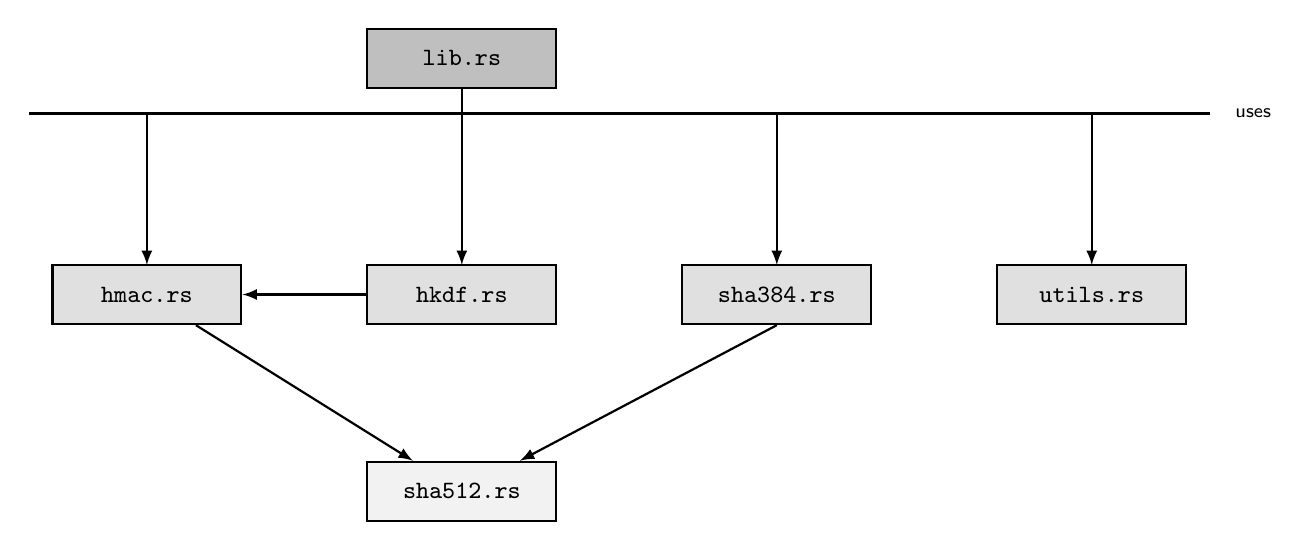
\begin{tikzpicture}[
			mod/.style={rectangle, draw=black, thick, minimum width=2.4cm, minimum height=0.75cm, align=center, font=\ttfamily\small},
			line/.style={draw, thick, -latex}
		]
		% Fasad
		\node[mod, fill=black!25] (lib) at (0, 6) {lib.rs};

		% Kurung horizontal
		\draw[thick] (lib.south) -- (0, 5.3);
		\draw[thick] (-5.5, 5.3) -- (9.5, 5.3);
		\node[font=\scriptsize\sffamily, anchor=west] at (9.7, 5.3) {uses};

		% Modul lapisan 1
		\node[mod, fill=black!12] (hmac)   at (-4, 3) {hmac.rs};
		\node[mod, fill=black!12] (hkdf)   at (0, 3) {hkdf.rs};
		\node[mod, fill=black!12] (sha384) at (4, 3) {sha384.rs};
		\node[mod, fill=black!12] (utils)  at (8, 3) {utils.rs};

		% Modul lapisan 0
		\node[mod, fill=black!5] (sha512) at (0, 0.5) {sha512.rs};

		% Panah dari kurung ke setiap modul lapisan 1
		\foreach \x in {-4, 0, 4, 8} {
				\draw[thick, -latex] (\x, 5.3) -- (\x, 3.375);
			}

		% Dependensi antar-modul
		\draw[line] (hmac) -- (sha512);
		\draw[line] (sha384.south) -- (sha512);
		\draw[line] (hkdf.west) -- (hmac.east);
	\end{tikzpicture}
	\caption{Struktur modul crate \texttt{libvctrl\_sha512}: \texttt{lib.rs} sebagai fasad menggunakan semua modul; \texttt{hmac} dan \texttt{sha384} bergantung pada \texttt{sha512}; \texttt{hkdf} bergantung pada \texttt{hmac}.}
	\label{fig:module-arch}
\end{figure}

Cara membaca Gambar~\ref{fig:module-arch}: gambar ini menampilkan \texttt{lib.rs} di bagian paling atas sebagai satu kotak. Dari bawah \texttt{lib.rs} keluar garis vertikal pendek yang langsung bercabang menjadi garis horizontal lebar (bracket). Dari bracket tersebut, empat panah pendek turun ke empat modul di baris kedua: \texttt{hmac.rs}, \texttt{hkdf.rs}, \texttt{sha384.rs}, dan \texttt{utils.rs}, tersusun dari kiri ke kanan. Di baris ketiga, hanya ada satu modul: \texttt{sha512.rs}, diletakkan di tengah. Tiga panah dependensi antar-modul ditambahkan: panah diagonal dari \texttt{hmac} ke \texttt{sha512}, panah diagonal dari \texttt{sha384} ke \texttt{sha512}, dan panah horizontal dari \texttt{hkdf} ke \texttt{hmac}. Semua panah mengalir satu arah dan tidak ada yang melintasi kotak lain. Inti pesan gambar ini adalah arsitektur dua lapis: fasad di atas, modul fungsional di tengah, dan \texttt{sha512} di dasar yang dipakai oleh dua modul.

\subsection{Feature Flags}

Crate ini punya dua feature flag. \texttt{sha384} (default) mengaktifkan modul SHA-384. \texttt{opt\_size} mengubah strategi inline pada round function SHA-512 untuk mengurangi ukuran binary.

\begin{lstlisting}[style=code]
[features]
default = ["sha384"]
sha384 = []
opt_size = []
\end{lstlisting}

Feature \texttt{sha384} bisa dinonaktifkan jika aplikasi hanya butuh SHA-512. Ini mengurangi waktu kompilasi dan ukuran binary sekitar sepuluh persen. Feature \texttt{opt\_size} berguna untuk target embedded dan WebAssembly, dengan trade-off performa sekitar lima belas persen lebih lambat.

\subsection{Dependency Policy}

Crate ini punya satu dependensi eksternal: \texttt{zeroize} versi 1.8 dengan \texttt{default-features = false}. Ini bukan dependensi runtime yang memerlukan sistem operasi; \texttt{zeroize} hanya menyediakan trait \texttt{Zeroize} dan wrapper \texttt{Zeroizing}, yang bekerja di \texttt{no\_std}.

Keputusan untuk mempertahankan dependensi seminimal mungkin adalah inti dari klaim auditabilitas crate. Setiap baris dependensi adalah baris yang harus diaudit. Dengan hanya \texttt{zeroize}, crate ini bisa diaudit secara menyeluruh oleh satu orang dalam beberapa hari.

\section{Perbandingan HMAC-SHA512, HMAC-SHA384, HMAC-SHA256}

\subsection{Perbedaan Utama}

Ketiga varian HMAC berbeda hanya pada fungsi hash yang dipakai, tetapi perbedaan ini membawa konsekuensi pada ukuran output, ukuran blok, dan performa.

\begin{table}[H]
	\centering
	\caption{Perbandingan tiga varian HMAC.}
	\label{tab:hmac-variants}
	\small
	\begin{tabularx}{\textwidth}{l r r r}
		\toprule
		Aspek             & HMAC-SHA512  & HMAC-SHA384  & HMAC-SHA256  \\
		\midrule
		Ukuran output     & 64 byte      & 48 byte      & 32 byte      \\
		Ukuran blok       & 128 byte     & 128 byte     & 64 byte      \\
		Jumlah round      & 80           & 80           & 64           \\
		Konstanta 0x6a    & ya           & ya           & ya           \\
		Panjang kunci max & tak terbatas & tak terbatas & tak terbatas \\
		Performa relatif  & tinggi       & tinggi       & sedang       \\
		Standar           & FIPS 180-4   & FIPS 180-4   & FIPS 180-4   \\
		\bottomrule
	\end{tabularx}
\end{table}

Ketiganya memakai konstanta \texttt{0x36} dan \texttt{0x5c} yang sama, sehingga trik transformasi \texttt{0x6a} berlaku universal. Yang berbeda hanya ukuran blok, yang mempengaruhi panjang array \texttt{padded} dan panjang array yang di-XOR.

\subsection{Kapan Memakai Apa}

HMAC-SHA512 cocok untuk aplikasi yang membutuhkan keamanan maksimum dan performa tinggi pada perangkat 64-bit. Ini termasuk penandatanganan token API, penandatanganan commit Git, dan autentikasi pesan jaringan.

HMAC-SHA384 cocok untuk aplikasi yang perlu kompatibilitas dengan standar yang lebih lama atau yang memiliki batas ukuran tag. Contohnya adalah suite cipher tertentu pada TLS 1.2 yang menggunakan SHA-384.

HMAC-SHA256 cocok untuk aplikasi yang dioptimalkan untuk perangkat dengan register 32-bit, karena SHA-256 lebih efisien di sana. Contohnya adalah perangkat IoT dengan CPU 32-bit.

Pada perangkat 64-bit modern, HMAC-SHA512 justru lebih cepat daripada HMAC-SHA256, karena operasi SHA-512 bekerja pada word 64-bit yang sesuai dengan lebar register.

\subsection{Interchangeability}

HMAC-SHA512 dan HMAC-SHA256 tidak saling menggantikan. Tag yang dihasilkan berbeda, ukuran output berbeda, dan blok yang diproses berbeda. Aplikasi yang menerima tag harus menyebutkan varian HMAC yang dipakai secara eksplisit.

Untuk kompatibilitas, banyak protokol menetapkan varian HMAC dalam negosiasi awal. Contohnya adalah TLS cipher suite yang menyebutkan varian PRF (pseudorandom function) secara eksplisit: \texttt{TLS\_ECDHE\_RSA\_WITH\_AES\_256\_GCM\_SHA384} memakai HMAC-SHA384 sebagai PRF.

\section{Studi Kasus: Implementasi HMAC-SHA512 dari Nol}

Bagian ini mengikuti sepuluh langkah mengimplementasikan HMAC-SHA512 dari nol, dengan setiap keputusan dijelaskan berdasarkan RFC 2104 dan perilaku crate \texttt{libvctrl\_sha512}.

\subsection{Langkah 1: Tentukan Parameter}

Parameter yang perlu ditentukan: fungsi hash (SHA-512), ukuran blok (128 byte), ukuran output (64 byte), dan konstanta padding (\texttt{0x36} dan \texttt{0x5c}).

\subsection{Langkah 2: Implementasikan SHA-512}

SHA-512 adalah inti dari HMAC-SHA512. Implementasi lengkap memerlukan inisialisasi state dengan IV 64 byte, fungsi kompresi 80 round, dan padding Merkle-Damgård. Untuk makalah ini, asumsikan SHA-512 sudah tersedia.

\subsection{Langkah 3: Implementasikan prepare\_key}

Fungsi \texttt{prepare\_key} menerima kunci berapa pun panjangnya dan mengembalikan array 128 byte. Tiga jalur: pendek, tepat, panjang.

\begin{lstlisting}[style=code]
fn prepare_key(key: &[u8]) -> [u8; 128] {
    let mut block_key = [0_u8; 128];
    if key.len() > 128 {
        let h = zeroize::Zeroizing::new(sha512(key));
        block_key[..64].copy_from_slice(&h[..64]);
    } else {
        block_key[..key.len()].copy_from_slice(key);
    }
    block_key
}
\end{lstlisting}

\subsection{Langkah 4: Bangun Inner State}

Inner hasher dimulai dengan memproses \texttt{ipad} yang sudah di-XOR dengan kunci.

\begin{lstlisting}[style=code]
let mut block_key = prepare_key(key);
let mut padded = [0x36_u8; 128];
for (p, k) in padded.iter_mut().zip(block_key.iter()) {
    *p ^= *k;
}
let mut ih = sha512_new();
ih.update(&padded);
zeroize::Zeroize::zeroize(&mut block_key);
\end{lstlisting}

Setelah langkah ini, \texttt{ih} sudah memproses 128 byte pertama (padat dengan \texttt{ipad} XOR K'). \texttt{block\_key} sudah di-zeroize.

\subsection{Langkah 5: Proses Pesan}

Setiap panggilan \texttt{update} meneruskan pesan ke inner hasher.

\begin{lstlisting}[style=code]
ih.update(&message);
\end{lstlisting}

Pesan bisa dipecah menjadi beberapa panggilan \texttt{update}, dan hasilnya akan sama dengan satu panggilan besar. Ini karena SHA-512 memproses input sebagai stream.

\subsection{Langkah 6: Transformasi 0x6a}

Sebelum memanggil outer hash, transformasikan \texttt{padded} dari \texttt{0x36 XOR K'} ke \texttt{0x5c XOR K'}.

\begin{lstlisting}[style=code]
for p in padded.iter_mut() {
    *p ^= 0x6a;
}
\end{lstlisting}

Satu baris mengubah seluruh array. Setelah loop ini, \texttt{padded} siap dipakai untuk outer hash.

\subsection{Langkah 7: Outer Hash}

Outer hasher dimulai dengan \texttt{padded} yang sudah ditransformasi, lalu memproses digest inner.

\begin{lstlisting}[style=code]
let mut oh = sha512_new();
oh.update(&padded);
let inner = zeroize::Zeroizing::new(ih.finalize());
oh.update(&*inner);
let tag = oh.finalize();
\end{lstlisting}

\subsection{Langkah 8: Verifikasi dengan Test Vector}

RFC 4231 menyediakan test vector untuk HMAC-SHA512. Test case 1 memakai kunci \texttt{0x0b} yang diulang 20 kali dan data \texttt{"Hi There"}. Tag yang diharapkan adalah sebagai berikut.

\begin{lstlisting}[style=out]
87aa7cdea5ef619d4ff0b4241a1d6cb0
2379f4e2ce4ec2787ad0b30545e17cde
daa833b7d6b8a702038b274eaea3f4e4
be9d914eeb61f1702e696c203a126854
\end{lstlisting}

Jika implementasi menghasilkan tag ini, implementasi berjalan benar.

\subsection{Langkah 9: Implementasikan Verify}

Verifikasi tag harus constant-time untuk mencegah timing attack.

\begin{lstlisting}[style=code]
fn verify(expected: &[u8], computed: &[u8]) -> bool {
    let mut diff: u32 = 0;
    for (a, b) in expected.iter().zip(computed.iter()) {
        diff |= u32::from(a ^ b);
    }
    if expected.len() != computed.len() {
        diff |= 0xffff_ffff;
    }
    diff == 0
}
\end{lstlisting}

\subsection{Langkah 10: Zeroization pada Drop}

Struct harus mengimplementasikan \texttt{Drop} untuk membersihkan state.

\begin{lstlisting}[style=code]
impl Drop for HMAC {
    fn drop(&mut self) {
        zeroize::Zeroize::zeroize(self);
    }
}
\end{lstlisting}

Setelah langkah ini, implementasi lengkap dan sesuai RFC 2104.

\subsection{Timeline Studi Kasus}

Gambar~\ref{fig:case-timeline} menampilkan sepuluh langkah sebagai **timeline horizontal** dengan kotak berlabel singkat yang bergantian atas dan bawah.

\begin{figure}[H]
	\centering
	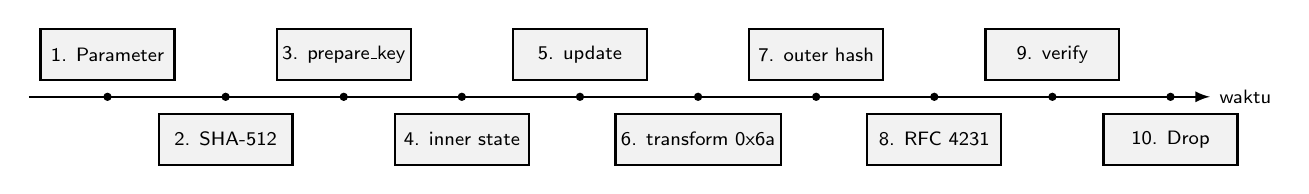
\begin{tikzpicture}[
			ev/.style={rectangle, draw=black, thick, fill=black!5, minimum width=1.7cm, minimum height=0.65cm, font=\scriptsize\sffamily, align=center, inner sep=2pt},
			dot/.style={circle, fill=black, inner sep=1.5pt}
		]
		% Garis waktu
		\draw[thick, -latex] (-7, 0) -- (8, 0);
		\node[font=\scriptsize\sffamily, anchor=west] at (8, 0) {waktu};

		% Titik-titik timeline
		\foreach \x in {-6, -4.5, -3, -1.5, 0, 1.5, 3, 4.5, 6, 7.5} {
				\fill (\x, 0) circle (1.5pt);
			}

		% Label bergantian atas dan bawah
		\node[ev, above=0.2cm] at (-6, 0) {1. Parameter};
		\node[ev, below=0.2cm] at (-4.5, 0) {2. SHA-512};
		\node[ev, above=0.2cm] at (-3, 0) {3. prepare\_key};
		\node[ev, below=0.2cm] at (-1.5, 0) {4. inner state};
		\node[ev, above=0.2cm] at (0, 0) {5. update};
		\node[ev, below=0.2cm] at (1.5, 0) {6. transform 0x6a};
		\node[ev, above=0.2cm] at (3, 0) {7. outer hash};
		\node[ev, below=0.2cm] at (4.5, 0) {8. RFC 4231};
		\node[ev, above=0.2cm] at (6, 0) {9. verify};
		\node[ev, below=0.2cm] at (7.5, 0) {10. Drop};
	\end{tikzpicture}
	\caption{Timeline sepuluh langkah implementasi HMAC-SHA512 dengan label bergantian atas-bawah.}
	\label{fig:case-timeline}
\end{figure}

Cara membaca Gambar~\ref{fig:case-timeline}: gambar ini menampilkan garis waktu horizontal dengan sepuluh titik hitam yang berjarak sama. Setiap titik diberi kotak label kecil yang bergantian posisi: titik ganjil (1, 3, 5, 7, 9) labelnya di atas garis, titik genap (2, 4, 6, 8, 10) labelnya di bawah garis. Isi label: Parameter, SHA-512, prepare\_key, inner state, update, transform 0x6a, outer hash, RFC 4231, verify, dan Drop. Semua kotak kecil dengan latar abu-abu sangat muda. Inti pesan gambar ini adalah urutan sepuluh langkah implementasi dari kiri ke kanan.

\begin{table}[H]
	\centering
	\caption{Ringkasan hasil studi kasus.}
	\label{tab:case-summary}
	\small
	\begin{tabularx}{\textwidth}{l X X}
		\toprule
		Langkah & Operasi                 & Hasil                             \\
		\midrule
		1       & tentukan parameter      & hash SHA-512, blok 128, output 64 \\
		2       & implementasikan SHA-512 & fungsi hash tersedia              \\
		3       & prepare\_key            & array 128 byte ternormalisasi     \\
		4       & inner state             & hasher siap menerima pesan        \\
		5       & update pesan            & state berisi ipad + pesan         \\
		6       & transformasi 0x6a       & padding berubah ke opad           \\
		7       & outer hash              & tag 64 byte dihasilkan            \\
		8       & verifikasi dengan RFC   & tag cocok dengan test vector      \\
		9       & verify constant-time    & perbandingan tanpa kebocoran      \\
		10      & zeroization pada drop   & state terhapus saat tidak dipakai \\
		\bottomrule
	\end{tabularx}
\end{table}

\section{Kesalahan Umum dan Cara Menghindarinya}

\begin{table}[H]
	\centering
	\caption{Kesalahan umum pada implementasi HMAC-SHA512.}
	\label{tab:mistakes}
	\footnotesize
	\begin{tabularx}{\textwidth}{l X X}
		\toprule
		Kesalahan                                        & Akibat                            & Perbaikan                          \\
		\midrule
		selalu hash kunci tanpa cek panjang              & tag tidak cocok dengan standar    & cek panjang, hash hanya jika > 128 \\
		tidak padding nol untuk kunci pendek             & tag salah untuk kunci < 128       & inisialisasi array dengan nol      \\
		ipad dan opad tertukar                           & tag valid untuk pesan lain        & ipad = 0x36, opad = 0x5c           \\
		transformasi 0x6a diaplikasikan sebelum update   & pesan rusak, tag salah            & transformasi hanya di finalize     \\
		tidak zeroize block\_key setelah new             & kunci tertinggal di stack         & panggil zeroize sebelum return     \\
		inner digest tidak di-zeroize                    & digest antara bisa bocor          & bungkus dengan Zeroizing           \\
		perbandingan tag dengan \texttt{==} biasa        & rentan timing attack              & pakai XOR akumulasi constant-time  \\
		kunci panjang tanpa \texttt{Zeroizing} pada hash & digest antara tertinggal di stack & bungkus hash dalam Zeroizing       \\
		tidak ada \texttt{Drop} untuk HMAC               & state tertinggal saat panic       & implementasikan \texttt{Drop}      \\
		finalize memakai \texttt{\&mut self}             & state bisa dipakai ulang          & finalize mengambil \texttt{self}   \\
		tidak menangani \texttt{None} dari \texttt{ih}   & panic saat update ganda           & pakai \texttt{unwrap\_or\_else}    \\
		tidak konsisten antara SHA-384 dan SHA-512       & kode kompatibilitas rusak         & pakai makro yang sama              \\
		\bottomrule
	\end{tabularx}
\end{table}

Dua kesalahan yang paling sering muncul adalah selalu hash kunci tanpa cek panjang dan tidak zeroize \texttt{block\_key} setelah konstruksi. Yang pertama membuat implementasi tidak kompatibel dengan standar. Yang kedua meninggalkan kunci di stack yang bisa bocor lewat memory disclosure.

\section{Lembar Rujukan Cepat}

\begin{table}[H]
	\centering
	\caption{Lembar rujukan cepat HMAC-SHA512.}
	\label{tab:cheat}
	\footnotesize
	\begin{tabularx}{\textwidth}{l X}
		\toprule
		Kebutuhan                 & Formula atau detail                                                        \\
		\midrule
		konstanta ipad            & \texttt{0x36} diulang 128 kali                                             \\
		konstanta opad            & \texttt{0x5c} diulang 128 kali                                             \\
		konstanta transformasi    & \texttt{0x6a} = \texttt{0x36 XOR 0x5c}                                     \\
		ukuran blok SHA-512       & 128 byte                                                                   \\
		ukuran output SHA-512     & 64 byte                                                                    \\
		ukuran blok SHA-384       & 128 byte                                                                   \\
		ukuran output SHA-384     & 48 byte                                                                    \\
		ukuran blok SHA-256       & 64 byte                                                                    \\
		ukuran output SHA-256     & 32 byte                                                                    \\
		normalisasi kunci pendek  & pad dengan \texttt{0x00} hingga 128 byte                                   \\
		normalisasi kunci tepat   & pakai apa adanya                                                           \\
		normalisasi kunci panjang & hash SHA-512 (64 byte), pad nol hingga 128 byte                            \\
		inner hash                & $H(\text{ipad} \oplus K' \parallel m)$                                     \\
		outer hash                & $H(\text{opad} \oplus K' \parallel \text{inner})$                          \\
		struktur HMAC             & $(K' \oplus \text{opad}) \parallel H((K' \oplus \text{ipad}) \parallel m)$ \\
		verifikasi tag            & XOR akumulasi seluruh byte                                                 \\
		mask WASM                 & hash akumulasi sebagai lapisan tambahan                                    \\
		zeroization block\_key    & setelah inner hasher diinisialisasi                                        \\
		zeroization inner digest  & setelah diserahkan ke outer hasher                                         \\
		zeroization padded        & via \texttt{Drop} saat HMAC keluar scope                                   \\
		test vector kunci pendek  & RFC 4231 Test Case 1                                                       \\
		test vector kunci panjang & RFC 4231 Test Case 6                                                       \\
		\bottomrule
	\end{tabularx}
\end{table}

\section{Kesimpulan}

HMAC-SHA512 adalah konstruksi autentikasi pesan yang telah terbukti secara formal dan dipakai secara universal. Dua mekanisme kunci dalam implementasinya adalah normalisasi kunci dan transformasi \texttt{0x6a}. Normalisasi kunci memastikan bahwa kunci berapa pun panjangnya diproses menjadi array 128 byte yang konsisten. Transformasi \texttt{0x6a} memastikan bahwa padding inner bisa diubah menjadi padding outer tanpa menyimpan salinan kunci.

Tiga prinsip penutup:

\begin{enumerate}
	\item Normalisasi kunci adalah persyaratan kompatibilitas. Implementasi yang tidak mengikuti tiga jalur \texttt{prepare\_key} akan menghasilkan tag yang tidak cocok dengan implementasi lain. Ini adalah bug paling sulit dideteksi karena hanya muncul pada kunci dengan panjang tertentu.
	\item Transformasi \texttt{0x6a} adalah konsekuensi aljabar. Konstanta \texttt{0x6a} bukan pilihan estetika, melainkan hasil XOR \texttt{0x36} dan \texttt{0x5c}. Memahaminya memungkinkan optimasi tanpa mengorbankan kompatibilitas.
	\item Verifikasi tag wajib constant-time. Perbandingan naif dengan \texttt{==} membocorkan informasi prefix yang cukup untuk melakukan timing attack. Untuk sistem yang terekspos jaringan, kebocoran ini bisa diselesaikan dalam hitungan detik.
\end{enumerate}

Pengembang yang memahami ketiga prinsip ini dapat mengimplementasikan HMAC-SHA512 yang kompatibel dengan standar, atau mengaudit implementasi yang sudah ada dengan mata yang lebih kritis.

\newpage
\section*{Referensi}
\addcontentsline{toc}{section}{Referensi}

\begin{thebibliography}{99}

	\bibitem{rfc2104}
	Krawczyk, H., Bellare, M., \& Canetti, R. (1997).
	\textit{HMAC: Keyed-Hashing for Message Authentication}.
	RFC 2104.
	IETF.
	\texttt{https://www.rfc-editor.org/rfc/rfc2104}

	\bibitem{rfc4231}
	Nystrom, M. (2005).
	\textit{Identifiers and Test Vectors for HMAC-SHA-224, HMAC-SHA-256, HMAC-SHA-384, and HMAC-SHA-512}.
	RFC 4231.
	IETF.
	\texttt{https://www.rfc-editor.org/rfc/rfc4231}

	\bibitem{nist-fips}
	National Institute of Standards and Technology. (2015).
	\textit{Secure Hash Standard (SHS)}.
	FIPS PUB 180-4.
	\texttt{https://doi.org/10.6028/NIST.FIPS.180-4}

	\bibitem{bellare1996}
	Bellare, M., Canetti, R., \& Krawczyk, H. (1996).
	Keying Hash Functions for Message Authentication.
	In \textit{Advances in Cryptology --- CRYPTO '96}
	(pp. 1--15). Springer.
	\texttt{https://doi.org/10.1007/3-540-68697-5\_1}

	\bibitem{bellare2006}
	Bellare, M. (2006).
	New Proofs for NMAC and HMAC: Security Without Collision-Resistance.
	In \textit{Advances in Cryptology --- CRYPTO '06}
	(pp. 602--619). Springer.
	\texttt{https://doi.org/10.1007/11818175\_36}

	\bibitem{rust-zeroize}
	The Rust Project Developers. (2026).
	\textit{zeroize: Securely clear secrets from memory}.
	docs.rs.
	\texttt{https://docs.rs/zeroize/}

	\bibitem{rust-nomicon}
	The Rust Project Developers. (2026).
	\textit{The Rustonomicon: The Dark Arts of Unsafe Rust}.
	\texttt{https://doc.rust-lang.org/nomicon/}

	\bibitem{rust-api-guidelines}
	The Rust Project Developers. (2026).
	\textit{Rust API Guidelines}.
	\texttt{https://rust-lang.github.io/api-guidelines/}

	\bibitem{libvctrl-sha512}
	Khafidi, M. R. (2026).
	\textit{libvctrl\_sha512: SHA-512, HMAC-SHA512, HKDF-SHA512}.
	docs.rs.
	\texttt{https://docs.rs/libvctrl\_sha512}

	\bibitem{libvctrl-source}
	Khafidi, M. R. (2026).
	\textit{libvctrl: A Precision Toolkit for Building Custom Version Control Systems}.
	GitHub.
	\texttt{https://github.com/mroczect/libvctrl}

	\bibitem{bernstein2005}
	Bernstein, D. J. (2005).
	\textit{Understanding Brute Force}.
	Chapter 5 in \textit{Introduction to Cryptography}.
	\texttt{https://cr.yp.to/papers.html}

	\bibitem{kocher1996}
	Kocher, P. C. (1996).
	Timing Attacks on Implementations of Diffie-Hellman, RSA, DSS, and Other Systems.
	In \textit{Advances in Cryptology --- CRYPTO '96}
	(pp. 104--113). Springer.
	\texttt{https://doi.org/10.1007/3-540-68697-5\_9}

	\bibitem{bernstein2005cache}
	Bernstein, D. J. (2005).
	Cache-Timing Attacks on AES.
	\textit{Technical Report}.
	University of Illinois at Chicago.
	\texttt{https://cr.yp.to/antiforgery/cachetiming-20050414.pdf}

	\bibitem{percival2009}
	Percival, C. (2009).
	\textit{Stronger Key Derivation via Sequential Memory-Hard Functions}.
	BSDCan 2009.
	\texttt{https://www.tarsnap.com/scrypt/scrypt.pdf}

\end{thebibliography}

\end{document}